\chapter{Open Habitats in the Lowlands}%
\label{ch:openhabitats}

At the time of European settlement some lowland areas, particularly in the North Island, were occupied by bracken fern or shrubland dominated by \IDX{manuka} (\BotanicRef{Leptospermum scoparium}[Leptospermum][scoparium]) and/or \IDX{kanuka} (\BotanicRef{Kunzea ericoides}[Kunzea][ericoides]).
It is now believed that these areas were originally largely under forest, which was destroyed and prevented from returning by repeated fires of both Maori and natural origin.
Many of the fires caused by the Maori were accidental, no doubt, but others were deliberate to encourage the growth of bracken fern whose rhizomes were an important source of starch.

Much of the eastern side of the South Island, as well as the Southland Plain, supported native grassland: short tussock grassland on the driest sites (the Marlborough Plains and adjacent hill country, the Canterbury Plains and foothills, and the Central Otago hill country) and tall tussock grassland of \IDX{red tussock} (\BotanicRef{Chionochloa rubra}[Chionochloa][rubra]) on the moister Southland plains and eastern Otago hills.
For some time it was assumed that the short tussock grassland was the original vegetation cover; the regions in which it predominated seeming too dry to support forest.
When exotic trees were planted and thrived, there must have been some doubt about this view, but it was not until relatively recent times that evidence came to light indicating that these areas of short tussock grassland originally supported forests and forest/tussock shrubland mosaics.
This evidence, to quote Molloy,\footnote{\cite{molloybpj1963distribution}} includes:

\begin{quote}
	surface logs and forest wind throw hummocks and hollows in now tree-less areas; buried wood, charcoal, and other plant remains; buried (forest) soil profiles; and a number of relict plants and soils.
\end{quote}

It is suggested that forests, particularly in the east of the country, became more susceptible to fire following a change to more variable climates with periodic droughts after about 1800 years ago.\footnote{\cite{mcglone1977ascarina}}

Identification of wood fragments has allowed a generalised reconstruction of these former Canterbury forests.\footnote{\cite{molloy1969recent}}
On the western ranges bordering the plains, beech forest extended in most places from tree line down to about \SI{1000}{\metre} altitude.
Below this, down to about \SI{400}{\metre}, came a mixed beech-podocarp forest, and on the plains themselves from \SI{300}{\metre} to sea level, there was a type of conifer broadleaf forest dominated by \IDX{matai} (\BotanicRef{Prumnopitys taxifolia}[Prumnopitys][taxifolia]) and \IDX{totara} (\BotanicRef{Podocarpus totara}[Podocarpus][totara]).
Near the sea on swampy sites were stands of \IDX{kahikatea} (\BotanicRef{Dacrycarpus dacrydioides}[Dacrycarpus][dacrydioides]) forest, of which Riccarton Bush is a surviving example.
Older, shallow soils were occupied by low forests of \IDX{kanuka} (\BotanicRef{Kunzea ericoides}[Kunzea][ericoides]), which may, in part at least, have resulted from natural fires.
Following the extensive destruction of the forests by fire during the period when the Maori was hunting moas in Canterbury, the higher altitude forests on the inland ranges were replaced by shrubland and \IDX{narrow-leaved snow tussock} (\BotanicRef{Chionochloa rigida}[Chionochloa][rigida]), which moved down from higher altitudes, and \IDX{red tussock} (\BotanicRef{Chionochloa rubra}[Chionochloa][rubra]) which moved out from poorly drained sites on to sometimes quite well-drained hillsides.
On the plains themselves, short tussock grassland became established:

\begin{quote}
	The species forming this grassland would have come largely from river and stream bed floras, from small enclaves of tussock within the forest, from the florulas of rock outcrops, and from among the species with short life-cycles from the alpine snow tussock above.\footnote{\cite{connor1969montane}}
\end{quote}

Short tussock grassland\figureref{\fullref{fig:81short-tussock}, \fullref{fig:82short-tussock}} is characterised by the light brown tufts, up to about half a metre high, of \IDX{hard tussock} (\BotanicRef{Festuca novae-zelandiae}[Festuca][novae-zelandiae]) together with \IDX{silver tussock} (\BotanicRef{Poa cita}[Poa][cita], previously \BotanicRef{Poa caespitosa}[Poa][caespitosa]), \IDX{blue tussock} (\BotanicRef{Poa colensoi}[Poa][colensoi]) and blue wheat grass (\BotanicRef{Elymus rectisetus}[Elymus][rectisetus]).
The most conspicuous shrub, particularly on stony, moister sites, is \IDX{matagouri} or `wild Irishman' (\BotanicRef{Discaria toumatou}[Discaria][toumatou])\figureref{\fullref{fig:83matagouri}}.
\IDX{Matagouri}[matagouri] is freely branched and interlaced and set with sharp spines that make it very unpleasant to push through.
Small leaves are produced in the spring, but the shrubs are quite leafless during the summer.

\begin{SCfigure}[2.0][!t]
	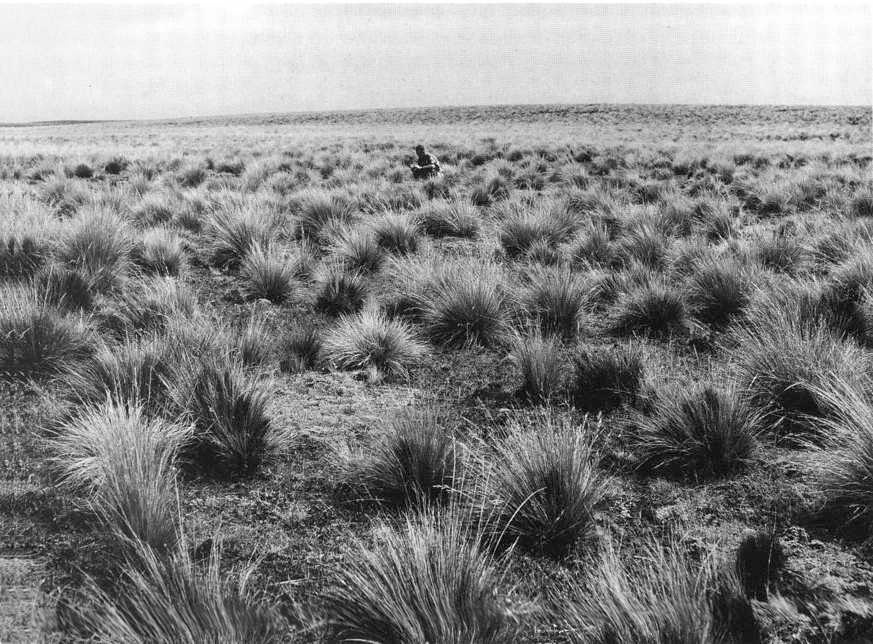
\includegraphics[width=0.66\textwidth]{graphics/figure81short-tussock.jpg}
	\centering
		\caption[Short tussock grassland dominated by fescue-tussock]{Short tussock grassland dominated by \IDX{fescue tussock} (\BotanicRef{Festuca novae-zelandiae}[Festuca][novae-zelandiae]) on the Mt. Hay Station, Tekapo, central South Island.
		Photo:  E. J. Godley.}%
		\label{fig:81short-tussock}
\end{SCfigure}
\begin{SCfigure}[2.0][!t]
	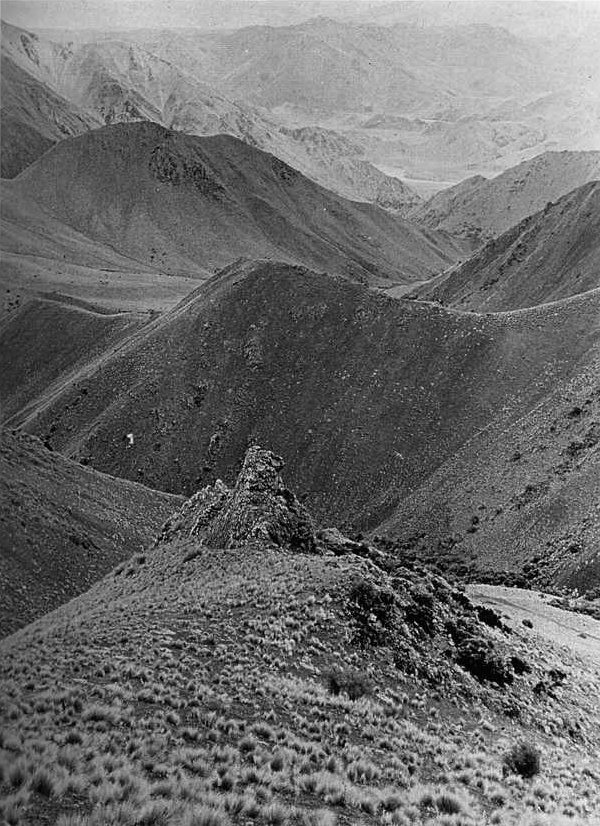
\includegraphics[width=0.66\textwidth]{graphics/figure82short-tussock.jpg}
	\centering
		\caption[Short tussock grassland mostly of \emph{Festuca novae-zelandiae}]{Short tussock grassland mostly of \IDX{fescue tussock} (\BotanicRef{Festuca novae-zelandiae}[Festuca][novae-zelandiae]) on hills north of the upper Waitaki River.
		Drought resistant shrubs grow on rock outcrops and along the bottoms of gullies where more moisture is available.  Photo:  J. W. Dawson.}%
		\label{fig:82short-tussock}
\end{SCfigure}
\begin{SCfigure}[2.0][t]
	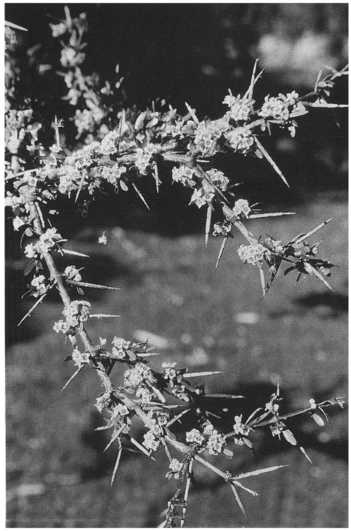
\includegraphics[width=0.33\textwidth]{graphics/figure83matagouri.jpg}
	\centering
	\caption[Matagouri]{\IDX{Matagouri}[matagouri] or `Wild Irishman' (\BotanicRef{Discaria toumatou}[Discaria][toumatou]) showing spines and flowers.
	Photo:  J. W. Dawson.}%
	\label{fig:83matagouri}
\end{SCfigure}

Two leafless \IDX{broom}s, \BotanicRef{Carmichaelia petriei}[Carmichaelia][petriei] and \BotanicRef{Carmichaelia robusta}[Carmichaelia][robusta], with slender switch-like branches, may stand above the tussocks in drier sites, while among smaller shrubs are \BotanicRef{Pimelea oreophila}[Pimelea][oreophila] and \IDX{patotara} (\BotanicRef{Styphelia nesophila}[Styphelia][nesophila] = \BotanicRef{Cyathodes fraseri}[Cyathodes][fraseri]).
Notable among the larger herbs is the spaniard\footnote{Also known as speargrass.} \BotanicRef{Aciphylla subflabellata}[Aciphylla][subflabellata], whose close rosettes of much-divided leaves look like clusters of grey, slender, sharply-pointed knitting needles and whose equally spiny bracts form cage-like enclosures for the seeds\figureref{\fullref{fig:84aciphylla}, \fullref{fig:85aciphylla-seedhead}}.
The \IDX{golden spaniard} (\BotanicRef{Aciphylla aurea}[Aciphylla][aurea]) also often descends into short tussock grassland from higher altitudes.

\begin{figure}[t]
	% Outer minipage scaled to limit width.
	% Inner minipages scaled so the images have the same height.
	\begin{minipage}[t]{\textwidth}
		\begin{minipage}[t]{(\textwidth-\fgap) * \real{0.523}}
			\centering
			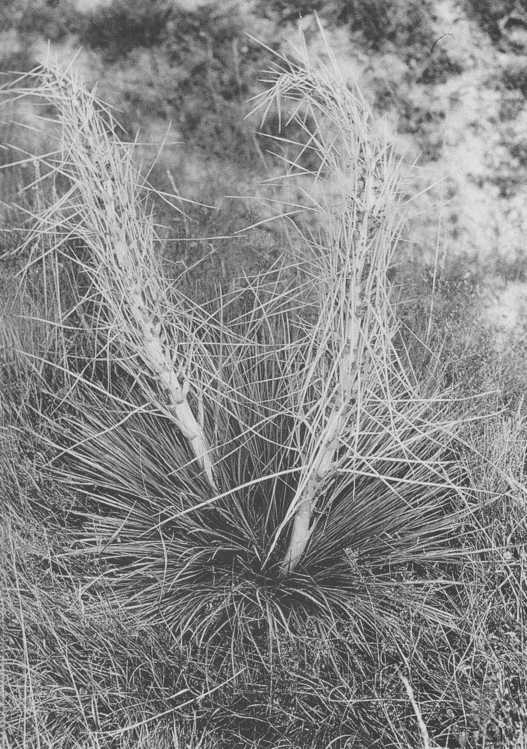
\includegraphics[width=\textwidth]{graphics/figure84aciphylla.jpg}
			\caption[\emph{Aciphylla subflabellata with male inflorescencs}]{\BotanicRef{Aciphylla subflabellata}[Aciphylla][subflabellata] with male inflorescences.
			Photo:  J. W. Dawson.}%
			\label{fig:84aciphylla}
		\end{minipage}\hspace{\fgap}%
		\begin{minipage}[t]{(\textwidth-\fgap) * \real{0.477}}
			\centering
			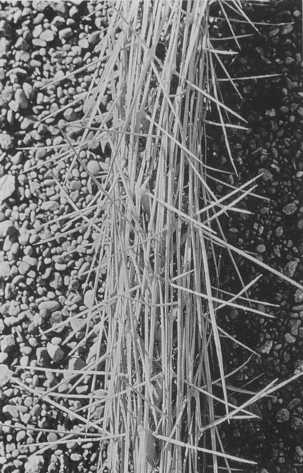
\includegraphics[width=\textwidth]{graphics/figure85aciphylla-seedhead.jpg}
			\caption[\emph{Aciphylla subflabellata} seedhead]{\BotanicRef{Aciphylla subflabellata}[Aciphylla][subflabellata] seedhead with most of the bract segments aligned vertically to form a cage around the seeds.
			Photo:  J. W. Dawson.}%
			\label{fig:85aciphylla-seedhead}
		\end{minipage}
	\end{minipage}
\end{figure}

One of the driest regions supporting short tussock grassland was the Central Otago hill country and here overgrazing with sheep and the later depredations of rabbits reduced the landscape to virtual desert\figureref{\fullref{fig:86barren}}.
The tussocks were largely replaced by grey patches of \BotanicRef{Raoulia australis}[Raoulia][australis], unflatteringly termed `\IDX{scabweed}'.

\begin{figure}[t]
	\centering
	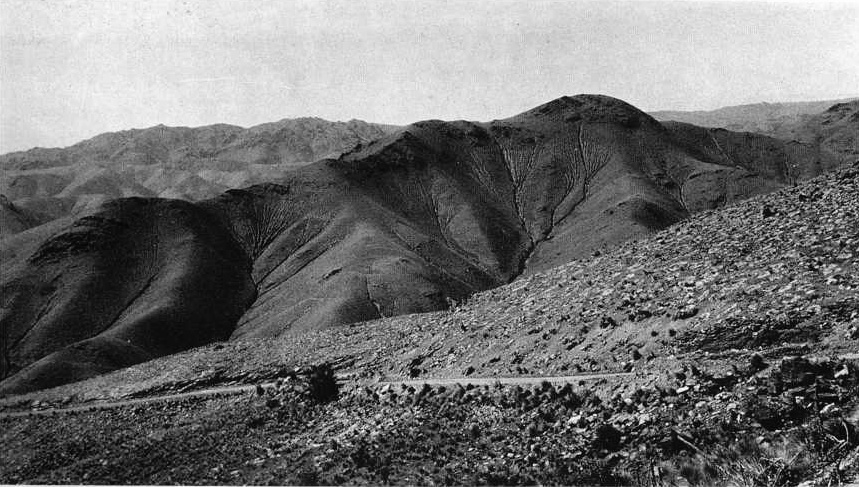
\includegraphics[width=\textwidth]{graphics/figure86barren.jpg}
	\caption[A barren landscape near Bannockburn]{A barren landscape near Bannockburn, Central Otago.
	The hillside in the foreground above the road has patches of `scabweed' (\BotanicRef{Raoulia australis}[Raoulia][australis]).
	Photo:  J. W. Dawson.}%
	\label{fig:86barren}
\end{figure}

Let us return to the \IDX{red tussock} grassland at the moister southern end of the South Island.
A recent study\footnote{\cite{mcglone1983vegetation}} of fossil pollen from bogs built up over the past 12000 years on the Longwood Range in Southland, indicates that forests also covered the southern end of New Zealand until about 1000 years ago.
The species represented suggest that \IDX{kahikatea} (\BotanicRef{Dacrycarpus dacrydioides}[Dacrycarpus][dacrydioides])-dominated forest occupied moister and swampy sites, \IDX{rimu} (\BotanicRef{Dacrydium} cupressinum)-dominated forest drier sites and \IDX{silver beech} (\BotanicRef{Nothofagus menziesii}[Nothofagus][menziesii]) forest the higher altitudes.

After 1000 B.P. (before present) the proportion of forest pollen decreased and spores of bracken fern and grass pollen increased.
After 700 B.P. there was a striking upsurge of bracken spores followed by a peak of grass pollen:

\begin{quote}
	We conclude that localised burning took place shortly after the arrival of Polynesians in Southland, which was followed some 200 years later by wholesale destruction of lowland forest by fire.
	Immediately after the destruction of the forests fernland established, but, with continued burning, grassland began to spread … The first European settlers found the Southland Plains in shrubland, fern, and tussock, with indications in some areas that succession back to high forest had begun.
\end{quote}

A similar sequence has been described from Lake Poukawa in the eastern North Island.\footnote{\cite{mcglone1978forest}}

Thus it seems that in their original state, before the increasing frequency of natural and human-caused fires over the past few thousand years, the lowlands of New Zealand had few sites not occupied by forests.
In such open habitats as there were, establishment of trees would have been precluded by some localised environmental factor: periodic flooding and disturbance of parts of riverbeds normally above water level; excessive salinity in some coastal sites; excessive drainage and sparse soil of cliffs and bluffs in the drier eastern part of the country, and the infertile soils, containing varying concentrations of toxic metals (nickel, chrome, magnesium), derived from the ultramafic rocks more commonly known as `serpentine'.

Lowland bogs and swamps would also have been treeless, but as these alter with time under the influence of plant cover and generally give way to forest, they have already been considered in Chapter~\ref{ch:coniferpatterns} \nameref{ch:coniferpatterns}.

\section{River Beds}

These vary in their form quite markedly depending on the amount of eroded material --- rock fragments, sand, silt --- being brought down from the mountains.
Where there is more material than the river can readily transport to the sea, the river bed is steadily raised.
At the other extreme, where eroded material is slight and there is a sufficient fall to the sea, the river steadily cuts down into its bed.
The best examples of the former type are the rivers traversing the Canterbury Plains\figureref{\fullref{fig:87rakaia}}.
\begin{figure}[t]
	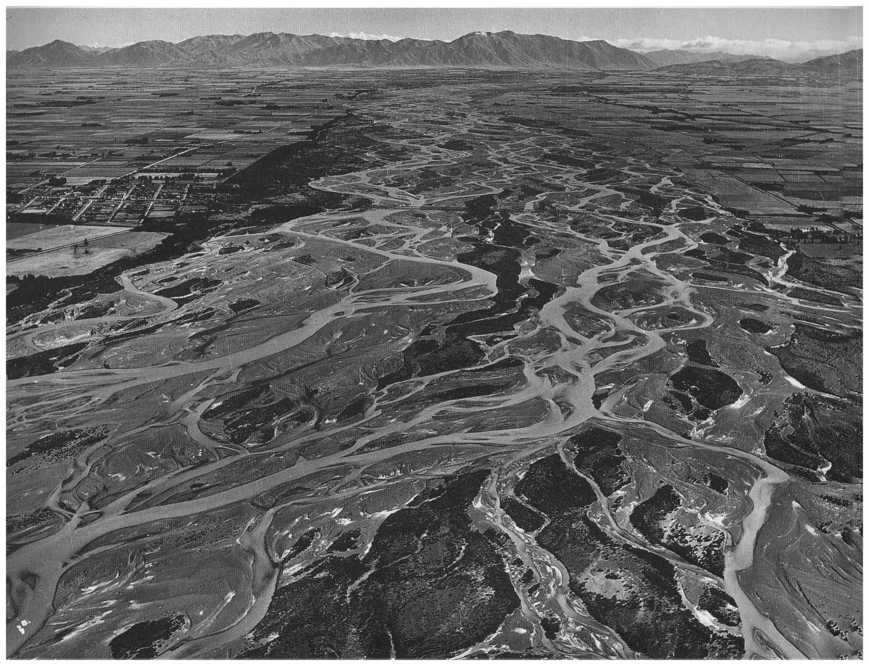
\includegraphics[width=\textwidth]{graphics/figure87rakaia.jpg}
	\centering
	\caption[The Rakaia River]{The Rakaia River, a typical braided river of the Canterbury Plains.
	Photo: V. C. Browne.}%
	\label{fig:87rakaia}
\end{figure}
These rivers have in fact built the Plains with the debris they have carried down from the Southern Alps.
Their beds are sometimes a few kilometres wide and are described as `braided' as they exhibit a network of channels, of which only a few actually carry water at any particular time.
As each water-filled channel builds up to a higher level than adjacent dry channels it may take only a slight freshening of water flow to divert the river into a new course at a lower level.
Such channel changes, and occasional floods which fill the river bed from bank to bank, put riverbed plants at a constant risk of being swept away.
When a portion of a riverbed has been stable and dry for a time plants begin to establish.
First come species of \BotanicRef{Epilobium}, \IDX{creeping willowherb} (\BotanicRef{Epilobium brunnescens}[Epilobium][brunnescens]), \IDX{willowherb} (\BotanicRef{Epilobium melanocaulon}[Epilobium][melanocaulon]) and \BotanicRef{Epilobium microphyllum}[Epilobium][microphyllum], and flat circular patches, up to a metre in diameter, of \IDX{tutahuna} (\BotanicRef{Raoulia tenuicaulis}[Raoulia][tenuicaulis]).
As wind-blown silt accumulates, \IDX{scabweed} (\BotanicRef{Raoulia hookeri}[Raoulia][hookeri]), \BotanicRef{Raoulia australis}[Raoulia][australis] and other epilobiums follow and, if stable conditions continue, taller plants appear: short tussock grasses, carmichaelias, hebes, parahebes, \IDX{matagouri} (\BotanicRef{Discaria toumatou}[Discaria][toumatou]) and others.\footnote{\cite{calder1961plant}}

Rivers that are cutting down have much narrower beds which are largely under water most of the time.
Such rivers are often confined by quite steep banks or, in gorges, by high cliffs.
Plants grow mostly on the banks or cliffs, although some may establish on `islands' in the bed itself.
Rivers of this type are quite common in the North Island and some parts of the South Island.

The alluvial flood plains beyond the river banks often support communities of small trees.
The species concerned are not confined to such sites, but some are most frequent there, including \IDX{manatu} (\BotanicRef{Plagianthus regius}[Plagianthus][regius], \IDX{ribbonwood}), and species of \IDX{lacebark} (\BotanicRef{Hoheria}) of the family Malvaceae and perhaps most notably the small trees that bear New Zealand's best known flower, the \IDX{kowhai}s (\BotanicRef{Sophora}).
\IDX{Small-leaved kowhai}[small-leaved kowhai] (\BotanicRef{Sophora microphylla}[Sophora][microphylla]) is found throughout and \IDX{large-leaved kowhai} (\BotanicRef{Sophora tetraptera}[Sophora][tetraptera]), with larger leaflets, in the eastern North Island.
The flowers, which are pollinated by birds, are golden yellow, pendent and more or less tubular in form.

On the rocky banks and lower parts of cliffs of the river bed itself plants are subjected to more frequent floods and are much smaller.
Common among herbaceous plants are ferns, including several species of \BotanicRef{Blechnum}, and flowering plants such as the small-leaved, creeping species of \BotanicRef{Gunnera} and the two subshrubby species of \BotanicRef{Jovellana}, a genus closely related to \BotanicRef{Calceolaria}.
Among shrubs several willow-leaved \IDX{koromiko}s (\BotanicRef{Hebe}) are prominent, for example \BotanicRef{Hebe salicifolia}[Hebe][salicifolia] and varieties of \BotanicRef{Hebe stricta}[Hebe][stricta], as well as several species of the related \BotanicRef{Parahebe} of which one is appropriately named \BotanicRef{Parahebe catarractae}[Parahebe][catarractae] (\IDX{Fiordland parahebe}).

A number of species of leafless \IDX{broom} (\BotanicRef{Carmichaelia}) are often encountered in these riverbeds.
They have slender but tough, flattened, more or less trailing stems with no leaves, or leaves for only part of the year.
In the tropics there are often distinct communities of shrubs growing within the flood zone of streams.\footnote{\cite{ansteenis1981rheophytes}}
Some of the species grow nowhere else and are `streamlined' with long, narrow leaves and tough, slender stems to minimise the force of the water during floods.
Probably none of the New Zealand species is restricted to river beds, but some show similar modifications to those in the tropics.
The narrow-leaved hebes look remarkably like the unrelated \BotanicRef{Metrosideros operculata}[Metrosideros][operculata] of New Caledonian stream beds and the carmichaelias with their modified stems seem well suited to avoiding damage from floods.
The species of \BotanicRef{Notospartium} and \BotanicRef{Chordospartium}, related to \BotanicRef{Carmichaelia}, of the north-eastern South Island, have `slender, drooping, leafless branches' and may also grow near rivers.

This leads to the speculation that in warmer Tertiary times when open, lowland habitats were in short supply, \BotanicRef{Hebe}, \BotanicRef{Parahebe}, and \BotanicRef{Carmichaelia} may have been largely confined to riverbeds, diversifying into other open habitats when forests retreated during glaciations.

\section{Cliffs and Rock Outcrops}

Inland river cliffs above flood level in moister areas support a number of distinctive species mostly with drooping leaves or stems.
The most striking and attractive of these, is the large-leaved fern \IDX{kiokio} (\BotanicRef{Blechnum capense}[Blechnum][capense]), which sometimes covers large areas to the exclusion of other plants.
Other species conspicuous at some localities are various willow-leaved \IDX{koromiko}s (\BotanicRef{Hebe}), the robust pendent sedge \BotanicRef{Machaerina sinclairii}[Machaerina][sinclairii], and, in better-lit places, the slender drooping stems of \IDX{ti ngahere} (\BotanicRef{Cordyline banksii}[Cordyline][banksii], \IDX{cabbage tree}).
\IDX{Parataniwha}[parataniwha] (\BotanicRef{Elatostema rugosum}[Elatostema][rugosum])\figureref{\fullref{fig:63parataniwha}} in northern parts of the country may cover with its attractive purplish foliage extensive areas of cliff, in the wettest and shadiest places.

Cliffs and rocky slopes along the coasts are populated by hardier species able to withstand gales and salt.\footnote{\cite{moore1963plants}}
In the most exposed situations low growing succulent plants predominate, including the native \IDX{ice plant} (\BotanicRef{Disphyma australe}[Disphyma][australe]), the \IDX{glasswort} \BotanicRef{Sarcocornia quinqueflora}[Sarcocornia][quinqueflora], \IDX{New Zealand celery} (\BotanicRef{Apium prostratum}[Apium][prostratum]) and \IDX{shore groundsel} (\BotanicRef{Senecio lautus}[Senecio][lautus]).
In the North Island particularly, prostrate shrubs of the shiny-leaved \IDX{taupata} (\BotanicRef{Coprosma repens}[Coprosma][repens], known as the `looking glass plant' in California where it is cultivated) are often prominent.
On more sheltered aspects, so-called mountain flax, \IDX{wharariki} (\BotanicRef{Phormium cookianum}[Phormium][cookianum]) may form a close cover, in association with \IDX{koromiko} (\BotanicRef{Hebe macroura}[Hebe][macroura]) in the East Cape region, \BotanicRef{Hebe stricta}[Hebe][stricta] in central New Zealand and, in the southern South Island and Fiordland, \IDX{kokomuka} (\BotanicRef{Hebe elliptica}[Hebe][elliptica]) and several ferns.

The drier inland and coastal cliffs of Marlborough have their own distinctive flora.
Notable is the genus \BotanicRef{Pachystegia} (Compositae) endemic to Marlborough and North Canterbury.
Until recently it was thought that there was only one species but a study in progress indicates that there could be as many as five.\footnote{\cite{molloy1980taxonomy}}
They are all small, spreading shrubs with thick, leathery leaves, densely furry beneath.
The flower buds are perhaps more striking than the flowers, being relatively large, almost globose and with many closely overlapping scale leaves.
They have been aptly likened to drumsticks.
Often associated with the Pachystegias, mostly at inland sites, are two other Marlborough and North Canterbury endemics, \IDX{Monro's groundsel} (\BotanicRef{Brachyglottis monroi}[Brachyglottis][monroi]) and \IDX{New Zealand lilac} (\BotanicRef{Hebe hulkeana}[Hebe][hulkeana]) with its freely branched inflorescences of small mauve flowers.
Other wider ranging shrubs are the dwarf \IDX{kowhai} (\BotanicRef{Sophora prostrata}[Sophora][prostrata]), the \IDX{leafless clematis} (\BotanicRef{Clematis afoliata}[Clematis][afoliata]), the densely twiggy \IDX{korokio} (\BotanicRef{Corokia cotoneaster}[Corokia][cotoneaster]) and other small, drought-resistant shrubs.
The latter group of species is also frequent on dry rocky outcrops further south in inland Canterbury and Otago.
On the south Otago coast, species of two predominantly alpine genera are conspicuous --- \IDX{Lindsay's daisy} (\BotanicRef{Celmisia lindsayi}[Celmisia][lindsayi]) on solid rock faces and stony debris and \IDX{Lyalls carrot} (\BotanicRef{Anisotome lyallii}[Anisotome][lyallii]) on debris.
Other forms of \BotanicRef{Anisotome lyallii}[Anisotome][lyallii] occur in Fiordland and Fiordland.

Also in Fiordland and Fiordland are distinctive coastal shrubberies of `daisy trees'.
These may overhang the sea or be separated from it by the \IDX{kokomuka} (\BotanicRef{Hebe elliptica}[Hebe][elliptica]) / \IDX{wharariki} (\BotanicRef{Phormium cookianum}[Phormium][cookianum]) association.
In more sheltered situations, \BotanicRef{Brachyglottis rotundifolia}[Brachyglottis][rotundifolia] predominates, with its large, round, leathery leaves giving way in exposed sites to \IDX{teteaweka} (\BotanicRef{Olearia angustifolia}[Olearia][angustifolia]), a handsome shrub with quite large, white, purple-centred flowers.

\section[Sand Dunes]{Sand Dunes\thinspace\footnote{\cite{moore1963plants}}}

Sandy beaches built up from the sea and backed by sand dunes that have been formed by wind are a feature of much of the coastline of both islands.
These beaches, regularly disturbed by tides, rarely support any plants and even the dune ridge immediately behind the beach is a difficult habitat for them.
The sand is unstable, frequently dry near the surface and with a high salt content from wind and spray.
A few plants however, known as sand binders, colonise such dunes and often completely cover them with foliage.
The sedge \IDX{pingao} (\BotanicRef{Desmoschoenus spiralis}[Desmoschoenus][spiralis], \IDX{golden sand sedge})\figureref{\fullref{fig:88pingao}}, now becoming rare, is the most robust and colourful of these with its coarse, narrow, curving leaves coloured yellow to orange-brown.
\begin{figure}[t]
	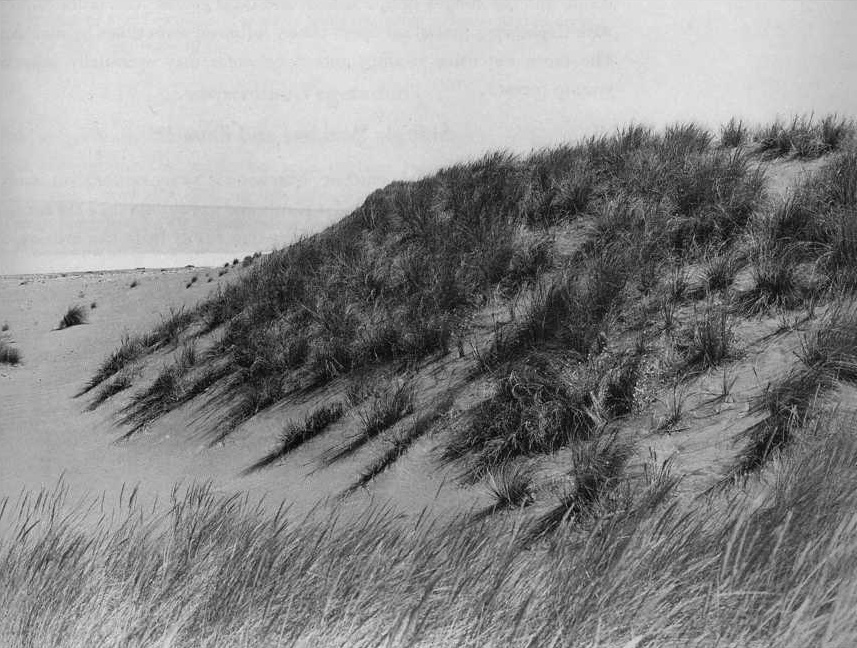
\includegraphics[width=\textwidth]{graphics/figure88pingao.jpg}
	\centering
	\caption[Robust leading shoots of pingao]{Robust leading shoots of \IDX{pingao} (\BotanicRef{Desmoschoenus spiralis}[Desmoschoenus][spiralis]) spreading through a sand dune.
	Photo: J. Miles.}%
	\label{fig:88pingao}
\end{figure}
It has widely spreading and branching subsurface rhizomes, which give rise to cord-like roots penetrating deep into the sandhill.
The silvery grass \IDX{kowhangatara} (\BotanicRef{Spinifex sericeus}[Spinifex][sericeus]) is equally common, but in this case the more slender rhizomes spread and branch over the surface of the sand.
The seed heads of \BotanicRef{Spinifex} are distinctive in that they bear quite long, spherically arranged, flexible spines, which enable the heads to bowl along with the wind over the beaches and dunes for considerable distances.
The introduced \IDX{marram grass} (\BotanicRef{Ammophila arenaria}[Ammophila][arenaria]) is now also common as a sand binder.

As a dune becomes consolidated by the sand binders and particularly when new sheltering dunes are formed seaward of it, other species less tolerant of instability enter in.
These include the herbaceous \IDX{native spinach} (\BotanicRef{Tetragonia trigyna}[Tetragonia][trigyna]) and the \BotanicRef{Convolvulus}-like \IDX{rauparaha} (\BotanicRef{Calystegia soldanella}[Calystegia][soldanella], \IDX{shore bindweed}); the low shrubs \IDX{autetaranga} or \IDX{toroheke} (\BotanicRef{Pimelea arenaria}[Pimelea][arenaria]) and \IDX{sand coprosma} (\BotanicRef{Coprosma acerosa}[Coprosma][acerosa]), which has interlaced mattress-like orangey stems bearing minute leaves.

Eventually a variety of taller shrubs, robust herbs and climbers common in open inland situations may form dense communities: \IDX{toetoe} (\BotanicRef{Cortaderia fulvida}[Cortaderia][fulvida]), \IDX{harakeke} (\BotanicRef{Phormium tenax}[Phormium][tenax]), species of leafless \IDX{broom} (\BotanicRef{Carmichaelia}), \IDX{matagouri} (\BotanicRef{Discaria toumatou}[Discaria][toumatou]), species of \BotanicRef{Cassinia}, \IDX{manuka} (\BotanicRef{Leptospermum scoparium}[Leptospermum][scoparium]), the introduced shrubby \BotanicRef{Lupinus arboreus}[Lupinus][arboreus] and others.
Given continuing stability and sufficient time a progression to forest can take place.

In the hollows between dunes, damp or even swampy conditions often prevail.
The first plants to establish in such moist and relatively sheltered situations are such small herbs as \BotanicRef{Gunnera arenaria}[Gunnera][arenaria], \IDX{sand buttercup} (\BotanicRef{Ranunculus acaulis}[Ranunculus][acaulis]) and the sedges IDX{wiwi} (\BotanicRef{Isolepis nodosus}[Isolepis][nodosus]) and \BotanicRef{Carex pumila}[Carex][pumila].
The taller \IDX{jointed wire rush}, \IDX{oioi} (\BotanicRef{Leptocarpus similis}[Leptocarpus][similis]) succeeds these, followed sometimes by \IDX{manuka}.
The more extensive swampy interdune areas may eventually support swamp forest.

\section[Shingle Beaches and Fans]{Shingle Beaches and Fans\thinspace\footnote{\cite{moore1963plants}}}

Along some parts of the coastline, beaches are stony rather than sandy.
They provide a more stable site for plants and as habitats they are similar to the sometimes adjacent shingle fans that result from the erosion of sea cliffs.

Nearest the sea are scattered succulent herbs such as \IDX{New Zealand celery} (\BotanicRef{Apium prostratum}[Apium][prostratum]) and \IDX{shore groundsel} (\BotanicRef{Senecio lautus}[Senecio][lautus]).
Further back we find larger herbs like \IDX{wharariki} (\BotanicRef{Phormium cookianum}[Phormium][cookianum]), the sedges \IDX{wiwi} (\BotanicRef{Isolepis nodosus}[Isolepis][nodosus]) and \IDX{coastal cutty grass} (\BotanicRef{Cyperus ustulatus}[Cyperus][ustulatus]), the white-flowered New Zealand species of true \IDX{linen flax}, \BotanicRef{Linum monogynum}[Linum][monogynum], and patches of the strange, leafless shrub, \BotanicRef{Muehlenbeckia ephedroides}[Muehlenbeckia][ephedroides].
On the terraces behind the beaches and on shingle fans there may be a close cover of densely twiggy, small-leaved shrubs belonging to several genera --- \IDX{mingimingi} (\BotanicRef{Coprosma propinqua}[Coprosma][propinqua]), \BotanicRef{Coprosma rigida}[Coprosma][rigida], \IDX{thick-leaved mahoe} (\BotanicRef{Melicytus crassifolius}[Melicytus][crassifolius]), \IDX{shrubby tororaro} (\BotanicRef{Muehlenbeckia astonii}[Muehlenbeckia][astonii]) and hummocky shrubby forms of the lianes \IDX{scrub pohuehue} (\BotanicRef{Muehlenbeckia complexa}[Muehlenbeckia][complexa]) and \IDX{leafless lawyer} (\BotanicRef{Rubus squarrosus}[Rubus][squarrosus]).
In this situation \BotanicRef{Rubus squarrosus}[Rubus][squarrosus] is quite leafless and beset with yellow prickles.
In the Cook Strait area the grey-leaved \IDX{spaniard} (\BotanicRef{Aciphylla squarrosa}[Aciphylla][squarrosa]) is also a common plant on fans.

\section[Salt Marshes and Meadows]{Salt Marshes and Meadows\thinspace\footnote{\cite{moore1963plants}}}

On sheltered low-lying coasts in muddy estuaries and lagoons, salt marshes frequently or occasionally flooded by tides, grade landwards into salt meadows rarely reached by the sea.
Nearest the sea, a zone that is under water for part of each day during spring tides has a close cover of the \IDX{glasswort} (\BotanicRef{Sarcocornia quinqueflora}[Sarcocornia][quinqueflora]).
Further from the sea and at a slightly higher elevation reached only by the highest spring tides, the next zone is dominated by taller rush-like plants including the true \IDX{sea rush} (\BotanicRef{Juncus maritimus}[Juncus][maritimus]) and the \IDX{jointed wire rush} (\BotanicRef{Leptocarpus similis}[Leptocarpus][similis]).
Often backing this zone is a fringe of the small-leaved twiggy shrub \IDX{marsh ribbonwood} (\BotanicRef{Plagianthus divaricatus}[Plagianthus][divaricatus]), a strange relative of the much larger \IDX{manatu} (\BotanicRef{Plagianthus regius}[Plagianthus][regius]) found in inland forests.
Furthest from the sea the salt meadow is rarely reached by the tide, but owes its moderate saltiness principally to salt-laden gales.
It has a turf of low-growing, mainly succulent herbs including \IDX{New Zealand celery} (\BotanicRef{Apium prostratum}[Apium][prostratum]), \IDX{remuremu} (\BotanicRef{Selliera radicans}[Selliera][radicans]) with its lobelia-like flowers, \IDX{sea primrose} (\BotanicRef{Samolus repens}[Samolus][repens]) and \IDX{shore cotula} (\BotanicRef{Leptinella dioica}[Leptinella][dioica], Cotula).
\BotanicRef{Triglochin striatum}[Triglochin][striatum] and \BotanicRef{Lilaeopsis} spp.\ are also common here.

\section{Serpentine Vegetation}

What is generally known as serpentine vegetation occurs in localised areas throughout the world on soils derived from ultramafic rocks.
These soils provide a difficult medium for plants, as they are highly infertile with low levels of potassium, phosphorus and calcium and often high concentrations of iron and magnesium and the toxic metals nickel and chrome.

As a result, in forested areas serpentine vegetation often has a very different appearance from the vegetation adjacent to or even surrounding it\figureref{\fullref{fig:89olivine-range}}.
\begin{figure}[!b]
	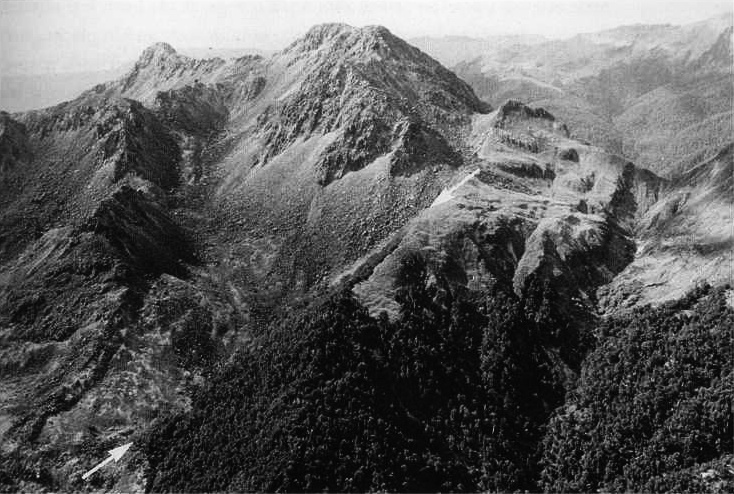
\includegraphics[width=\textwidth]{graphics/figure89olivine-range.jpg}
	\centering
	\caption[View of the Olivine Range]{View of the Olivine Range showing a contact between ultramafic rock (left) and schist (right).
	On the schist there is the normal forest to alpine vegetation sequence, on the ultramafic rock this is absent and there is a sparse cover of shrubs and herbs without a clear altitudinal zonation.
	Photo: P. F. Newsome.}%
	\label{fig:89olivine-range}
\end{figure}
The serpentine vegetation is more open with fewer, somewhat stunted trees and more shrubs and herbs.
Some of the species on serpentine, although often reduced in stature, are shared with non-serpentine forests, shrublands and grasslands; others are unique and are known as serpentine endemics.

In the South Island there is a belt of ultramafic rock, known as the `mineral belt', which runs through D'Urville Island, then to the east of Nelson and ends south of the Wairau River.\footnote{\cite{betts1918notes}}
A similar belt is found far to the south at the northern fringes of Fiordland.
The two belts are considered to have been continuous at one time until separated by lateral movement along the alpine fault.

In the North Island the only occurrences of ultramafic rock are at the northern tip along a few kilometres of the Surville Cliffs near North Cape and at the tip of the Peninsula a little to the south.

The serpentine flora at the Surville Cliffs has been investigated recently and 144 species have been recorded.\footnote{\cite{druce1979indigenous}}
Two unnamed shrub species of \BotanicRef{Hebe} and \BotanicRef{Coprosma} are considered to be endemic as well as 10 varieties, mostly of shrubs.
There are patches of low forest on the cliffs comprising common local species of which \IDX{pohutukawa} (\BotanicRef{Metrosideros excelsa}[Metrosideros][excelsa]) is the dominant.
Elsewhere the cover consists mainly of low shrubs draped with the string-like stems of the parasitic \IDX{taihoa} (\BotanicRef{Cassytha paniculata}[Cassytha][paniculata]).
The only conspicuous herbs are a \IDX{toetoe} (\BotanicRef{Cortaderia splendens}[Cortaderia][splendens]), \IDX{shore kowharawhara} (\BotanicRef{Astelia banksii}[Astelia][banksii]) and \IDX{harakeke} (\BotanicRef{Phormium tenax}[Phormium][tenax]).

A curious feature of a number of the shrubs at this locality is their `semi-lianoid' habit.
Their `elongated stems do not climb, but scramble or trail down the cliffs through other plants'.
Most of the shrubs exhibiting this habit are considered to be varieties of wider ranging species.

\section[The Effects of European Settlement]{The Effects of European Settlement\thinspace\footnote{\cite{healy1980flora}}\footnote{\cite{healy1969adventive}}}

This book is largely concerned with the native flora of New Zealand which has been evolving here for many millions of years.
Changes brought about by Europeans, in particular the establishment of introduced plants or `adventives', has occupied just a moment of geological time.
It is appropriate to consider these recent changes in this chapter as they tend to involve lowland open habitats.

A major aim of the European settlers was to establish farms, particularly sheep farms for the production of wool and meat.
Naturally the grasslands of the eastern South Island and southern North Island were exploited first, since there was no forest to be cleared and less possibility of conflict with the Maori, whose numbers were lower in the South Island.

The initial development of sheep runs on the natural grasslands took place from the 1840s to the 1860s.
At first the sheep were grazed on the native grasses, but as these were mostly coarse and not very palatable a practice developed of periodically setting fire to the grassland to induce soft new growth from the tussocks.
This resulted in loss of humus and reduced the fertility of the soil, so eventually the degraded short tussock grasslands of the Canterbury Plains and parts of Otago were replaced with European pasture grasses or grain crops.

In the higher country burning continued, and this, combined with overgrazing and the depredations of other introduced animals, particularly the rabbit, led to degeneration of the native vegetation.
In places, tall tussock grassland changed to short tussock grassland, and elsewhere short tussock grassland became virtual desert.
The situation has improved somewhat in recent years with the cessation of burning and the control of rabbits.

After the end of the New Zealand Wars in the North Island in the 1870s, extensive forest clearance began.
In the north, the main purpose was to obtain valuable construction timber from the forests containing \IDX{kauri}.
Elsewhere, obtaining timber was secondary to land clearance for sheep or dairy farming, and the forests were often destroyed by fire.

The fernlands and shrublands of the eastern North Island were also cleared for farming, but this was not successful on the volcanic plateau until the cobalt deficiency of the soil was corrected.
In this region extensive plantations of exotic pines have been and are still being established.

As the higher mountain areas are unsuitable for human settlement, it might be expected that the alpine vegetation there would have been little altered since the arrival of human beings.
It has been less altered, certainly, but introduced wild animals, notably deer and in places goats and thar, have reduced palatable species and interfered with natural regeneration.
As with the rabbits at lower elevations, some success has been achieved in controlling the numbers of these animals, particularly since the advent of deer hunting by helicopter.
In places in the mountains some alpine plants which had become rare are now re-establishing.

Deer have also been a problem in the forests, as has the introduced Australian opossum, which may entirely defoliate some palatable species such as \IDX{northern rata} (\BotanicRef{Metrosideros robusta}[Metrosideros][robusta]) and \IDX{whauwhaupaku} (\BotanicRef{Pseudopanax arboreus}[Pseudopanax][arboreus], \IDX{five-finger}).

Since European settlement a considerable number of plants from other countries, most notably Europe, have been deliberately or accidentally introduced.
Some of these have established themselves in the wild, mainly in the settled lowlands, and are known as the adventive flora.
Many of the adventives are herbaceous, often annual weeds of disturbed and waste places, and are not individually conspicuous.
Some cover more extènsive areas and may form pure associations.
Examples are gorse, particularly about Wellington; blackberry and \IDX{broom} in many areas; lupin on sand dunes; california thistle and ragwort in cultivated areas; nassella tussock in North Canterbury; sweet briar and sheep's sorrel on the drier eastern South Island; thyme in Central Otago; and in the northern North Island water hyacinth, which is presenting a problem by blocking streams and lakes.
The more cold-tolerant water weeds \BotanicRef{Elodea} and \BotanicRef{Lagarosiphon} appear to be spreading through both islands.

The adventives seemed so aggressive and successful that some early observers feared that the native flora was endangered.
Armstrong\footnote{\cite{armstrong1872naturalised}} wrote:

\begin{quote}
	The rapidity with which foreign plants become naturalised in New Zealand is indeed a most surprising and extraordinary circumstance, as it must be quite evident to every observer that the introduction of these European plants will certainly result in the extermination of the indigenous flora, and that at no distant period of time.
\end{quote}

Cockayne\footnote{\cite{cockayne1967plants}} disagreed with this view.
He considered that few adventives were successful where native vegetation was well established.
This is still generally the case.
Examples of the few exceptions are Scottish heather, which is well established in Tongariro National Park, and \IDX{lodgepole pine} (\BotanicRef{Pinus contorta}[Pinus][contorta]), which is an increasing problem in the same area.
